\chapter{Theory and related work}\label{ch:related}
This chapter describes the theoretical concepts that are required to understand this thesis and provides an overview of several related areas of research in the context of improving character recognition of steel type plates. It also provides an outline of current research done in the use of GANs for character recognition. 

\section{Introduction to deep learning}
	 
\begin{wrapfigure}{r}{0.5\textwidth}
\centering
\includegraphics[width=0.4\textwidth]{images/introdl.eps}
\caption[DL vs ML vs AI]{DL vs ML vs AI. Source: Adapted from \citep{aidlml} }
\label{fig:relation}
\end{wrapfigure}

\gls{dl} is a field of AI made up of neural networks inspired by the structure and function of the human brain. AI is growing at a rapid pace and deep learning is one of the major contributors to it. Deep learning is continuously changing the world around us. Its application ranges from speech recognition to driverless cars.

Figure \ref{fig:relation} shows the relationship between DL, ML and AI.
\textbf{Artificial Intelligence} is the branch of computer science that makes the computer mimic human intelligence such as visual perception, voice recognition, translation between languages and decision making.

\textbf{Machine Learning} is the subset of AI that enables the computer to learn to do a task on its own without explicitly telling it how to accomplish the task.

\textbf{Deep Learning} is the subfield of \gls{ml}, which deals with algorithms to train models like object detection and speech recognition using a multi-layered neural network with a vast amount of data. According to \citep{lecun2015deep},
“Deep learning allows computational models that are composed of multiple processing layers to learn representations of data with multiple levels of abstraction”. 
\subsection{Neural networks}

Figure \ref{fig:snn} shows the structure of a simple neural network. An \gls{ann} usually consists of an input layer, n number of hidden layers and an output layer. The input layer receives the input and sends it to the hidden layer. The hidden layer is responsible for processing the input and extracting the features, which is then passed onto the output layer. Each layer contains several neurons, and the neurons in each layer are connected to all the neurons in the next layer. 
\begin{figure}[H]
\centering
\includegraphics[width=3in]{images/nn.eps}
\caption[A simple neural network]{A simple neural network. Source: Created using tool \citep{nn}}
\label{fig:snn}
\end{figure}
\subsubsection*{Neuron}
Neurons, commonly known as nodes, are the basic building blocks of neural networks. A neuron receives input along with weights \& bias, and after processing, outputs the result as shown in Figure \ref{fig:Components of a neuron}. The output of a neuron is either used as the input to neuron in the next layer, or as the final output. 
\begin{figure}[H]
\centering
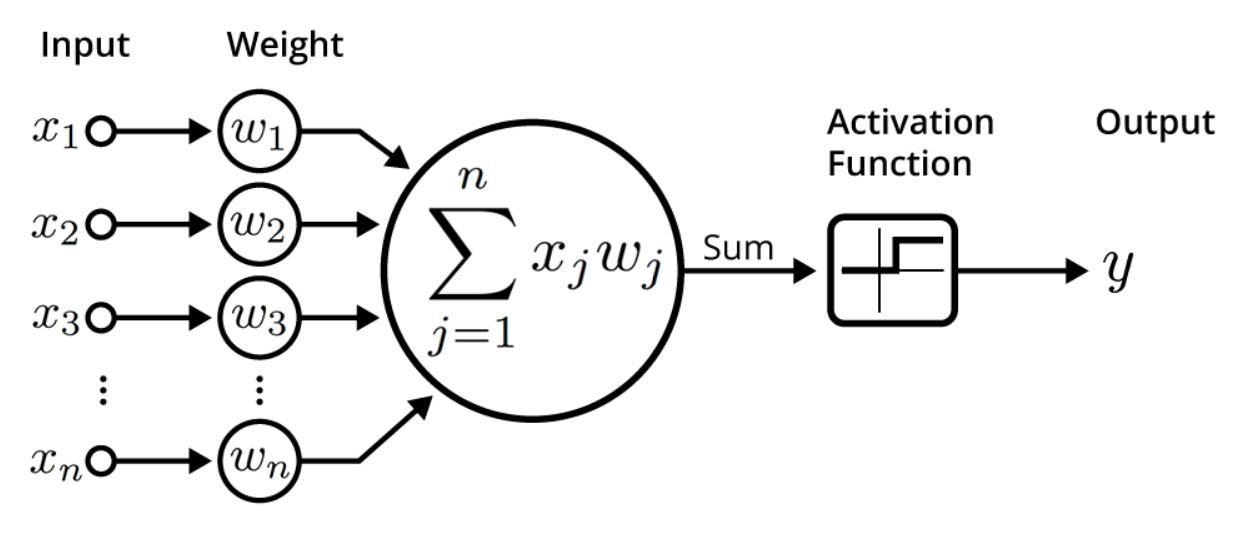
\includegraphics[width=4in,scale=1]{images/neuron.jpg}
\caption[Components of a neuron]{Components of a neuron. Source: \citep{neuron}}
\label{fig:Components of a neuron}
\end{figure}	
The output of a neuron can be mathematically represented as 
\begin{equation*}
Y=\sum_{j=1}^{n}w_{j}*x_{j} + b
\end{equation*}
	where w is the weight and b is the bias 	


\subsubsection*{Weights}

When the input data is passed into the neuron, a random weight is assigned to each information, and then the input information is multiplied by the corresponding weight. During training, the weight of each information is updated according to the corresponding feedback. 

\subsubsection*{Bias}

Bias is used as a constant to adjust the output along with the weighted sum of input in order to best fit the given data. It is added along with the result of the product of inputs and weights in the network. 

\subsubsection*{Activation function}
      The activation function converts an input signal of the neuron into any desired output signal. It is introduced to bring non-linearity into the network. The most common activation functions are sigmoid, \gls{relu}, tanh and softmax which are shown in Figure \ref{fig:activation functions}. 
\begin{figure}[H]
\centering
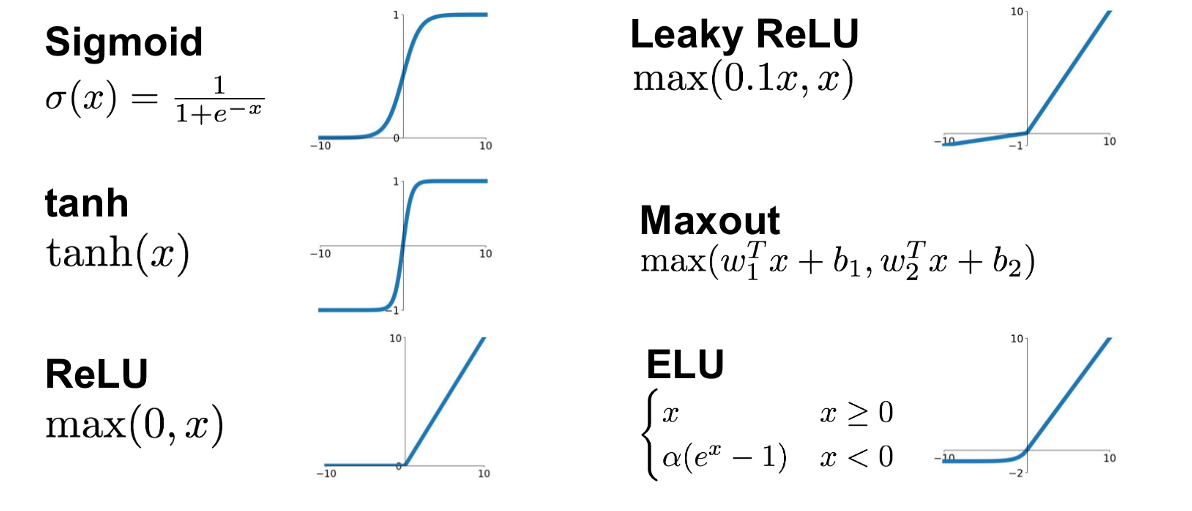
\includegraphics[width=4in,scale=1]{images/activation.png}
\caption[Different activation functions]{Different activation functions. Source: \citep{activation}}
\label{fig:activation functions}
\end{figure}
The final output of a neuron is given by
\begin{equation*}
      Y=\phi(\sum_{j=1}^{n}w_{j}*x_{j} + b)
\end{equation*}	
where $\phi$ can be any of these activation functions.

\subsection{Loss function and optimizer}
When training a neural network, the goal is to make the prediction as close as possible to the ground truth. The accuracy of the network is measured using the loss function. One of the most commonly used loss function is Mean Square Error (MSE). During training, the network makes use of loss value to adjust the weights so that the error is reduced at each iteration. 

\begin{equation*}
      MSE =\sum_{n}(y - \widehat{y})^2
\end{equation*}

where y is the ground truth and $\widehat{y}$ is the predictions.
\newline

	Optimizers are used to minimize the error calculated from the loss function. The most common optimization algorithm is gradient descent. \cite{kingma2014adam} proposed \gls{adam} optimizer which is the current benchmark optimizer for training deep learning models. It combines the Adagrad and RMSProp algorithm for better computational efficiency and memory requirements.

\subsection{Backpropagation}

The weights and biases in a neural network are learnable parameters. At first, when the neural network is built, they are randomly initialized. At each iteration, the network error is calculated by the forward propagation, and then to minimize the error, the gradients of the loss function are calculated and fed back to the network to update the weights \& biases in the network. This is called backpropagation.

\subsection{Hyperparameters}
 	Hyperparameters are the parameters that are not learnable during training a neural network. Some of the most common hyperparameters in deep learning are
\begin{enumerate}[(i)]
\item \textbf{Learning rate:} It is denoted by $\alpha$ that determines how fast the algorithm converges. If the learning rate is too high, it will overshoot the minima and if it is very low, the convergence will need more steps. Ideally, the learning rate is set between 0.0001 to 0.01.
\item \textbf{Regularization:} Regularization is the technique to avoid the overfitting of the model. The regularization parameter is denoted by $\lambda$. Dropout is used as a regularizer in neural networks. It refers to the training process of discarding a certain number of neurons present in the hidden layers of the network.
\begin{figure}
\centering
\includegraphics[width=4in,scale=1]{images/dropout.eps}
\caption[Effect of dropout]{Effect of dropout. Source: \citep{srivastava2014dropout}}
\label{fig:Dropout}
\end{figure}
\item \textbf{Batch size:} While training the neural network, instead of sending the entire input at once, the input is divided into several blocks of equal size called batches. In simple words, batch size determines the number of training examples present in a batch.
\item \textbf{Epoch:} An epoch is when the entire training data is propagated forward and backward through the neural network once.
\end{enumerate}

\section{Convolution Neural Networks}
\gls{cnn} is a type of deep neural network that is most commonly used for image recognition and classification. CNNs have been proven successful in various computer vision tasks like object detection, traffic sign detection, face recognition, scene text recognition, etc. The hidden layers \citep{Goodfellow-et-al-2016} in the CNN can be divided into convolutional layers, pooling layers, ReLU layers and fully connected layers as shown in Figure \ref{fig:cnn}.
\newline
\begin{figure}[H]
\centering
\includegraphics[width=4in,scale=1]{images/CNN.eps}
\caption[A CNN for MNIST handwritten recognition]{A CNN for MNIST handwritten recognition. Source: \citep{cnn}}
\label{fig:cnn}
\end{figure}

\subsection*{Convolution}

The operation of convolution layer starts with a kernel filter, which is just a small weight matrix. The kernel slides on the input data, multiplies the elements of the current input, and then summarizes the results into a single output pixel. The kernel repeats this process for each position in the image it slides over, transforming the input matrix into another feature matrix. The kernel filter values are randomly initialized and learnt during training.
\newline	
\begin{figure}[H]
\centering
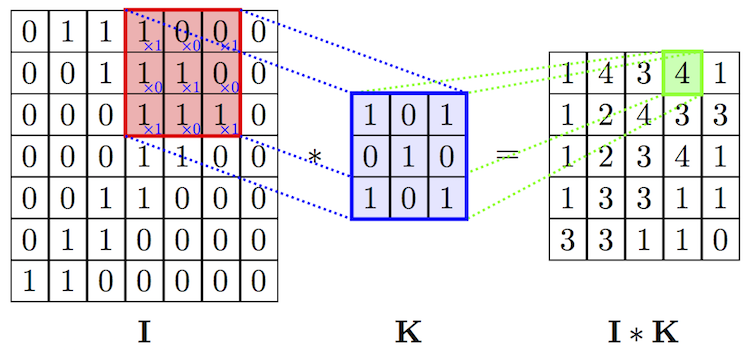
\includegraphics[width=3in,scale=.75]{images/convolution.png}
\caption[Convolution operation]{Convolution operation. Source: \citep{convolution}}
\label{fig:convolution}
\end{figure}
Generally, an image has a shape of C x H x W where C is the number of channels of an image(for RGB, C=3), H and W are the height and width of the image. The CNN layer consists of a kernel or a filter K with x rows, y columns and depth d. The result of the convolution \citep{cnneqn} of an image I with a kernel K with d channels is given by

\begin{equation*}
Conv(I,K)\textsubscript{xy}=\sum_{i=1}^{h}\sum_{j=1}^{w}\sum_{k=1}^{d}k_{ijk}.I_{x+i-1,y+j-1,k}
\end{equation*}
\subsection*{Pooling}
After the filter passes through the image, a feature map is generated for each filter. These functions are then obtained through activation functions, which determine whether a feature exists at a given location in the image. Then we can do a lot of things, such as adding more filter layers and creating more feature maps. As we create deeper CNNs, these maps become more and more abstract. We can also use pooling layers to select the maximum values or average values on the feature map and use them as input for subsequent layers.
\newline	
\begin{figure}[H]
\centering
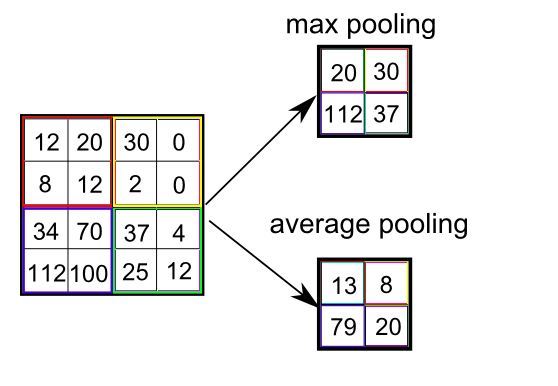
\includegraphics[width=3in,scale=.75]{images/maxpooling.png}
\caption[Pooling operation]{Pooling operation. Source: \citep{cnn}}
\label{fig:pooling}
\end{figure}

\subsection*{Fully connected layer}
This layer is similar to the conventional neural network, and its role is to fully connect the features obtained through multiple convolutional layers and multiple pooling layers and calculate the final predicted value. As the name implies, each neuron in this layer will be connected to all the nodes in the previous layer.
\subsection*{Normalization layer}
The normalization layer is used to normalize the activations in a neural network to give them a mean of 0 and a variance of 1. This thesis utilizes three normalization techniques i) Batch normalization, ii) Instance normalization and iii) Spectral normalization. 
\begin{enumerate}
\item \textbf{Batch normalization:} Generally the data should be normalized to make its distribution consistent. But during the training process of the deep neural networks, the data is fed into the network as batches and each batch has a different distribution. Hence \cite{ioffe2015batch} proposed batch normalization to make the distribution consistent and to reduce internal covariate shift.
\begin{figure}[H]
\centering
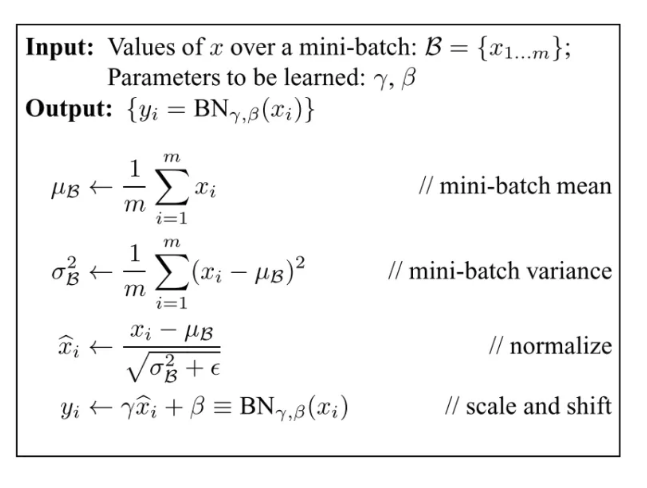
\includegraphics[width=4in,scale=1]{images/bnn.png}
\caption[Batch normalization algorithm]{Batch Normalization algorithm. Source: \citep{ioffe2015batch} }
\label{fig:bn}
\end{figure}
\item \textbf{Instance normalization:} The batch normalization doesn’t work well in distributed training in the case of multiple \gls{gpu}. Also, it focuses on normalizing each batch to ensure consistent data distribution. However, in image stylization, the generation result mainly depends on an image instance, so normalizing the entire batch is not suitable for image stylization. Hence, \cite{ulyanov2016instance} proposed instance normalization method normalizes only the height and width of the image. Thus it can accelerate model convergence and maintain independence between each image instance.
\begin{figure}[H]
\centering
\hspace*{1cm}\includegraphics*[width=5in,scale=1]{images/instancenorm.png}
\label{fig:ins}
\end{figure}
where x ∈ $\mathbb{R}$\textsuperscript{T×C×W×H} is the input tensor with a batch of T images and x\textsubscript{tijk} is its tijk-th element, where j and k are the dimensions, i is the feature/color channel and t is the image index in the batch \citep{ulyanov2016instance}.

\item \textbf{Spectral normalization:}
To improve the training stability of the discriminators and mitigate the problem of gradient explosion, \cite{miyato2018spectral} proposed a method called spectral normalization. It normalizes the weight for each layer of the network such that its Lipschitz constant always stays equals to one.
\end{enumerate}	

\section{Generative Adversarial Networks}
\cite{goodfellow2014generative} proposed GANs which is a type of deep neural network that generates data close to the input data distribution. The GAN network consists of two networks, Generator G and Discriminator D. These two neural networks compete against each other to learn the probability distribution of the dataset. The generator network learns to produce realistic samples and the discriminator learns to distinguish real data and samples produced from the generator. 
\begin{figure}[H]
\centering
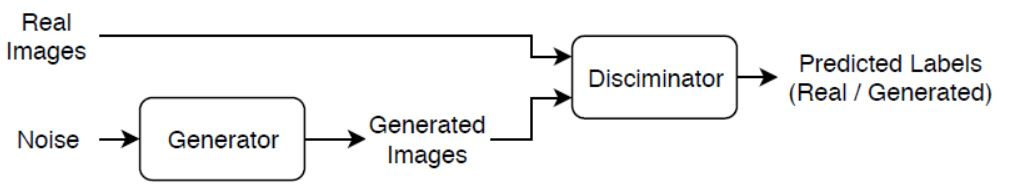
\includegraphics[width=5in]{images/GAN.jpg}
\caption[Generative Adversarial Network (GAN)]{Generative Adversarial Network (GAN). Source: \citep{gans}}
\label{fig:gan}
\end{figure}


In Figure \ref{fig:gandist}, the black dotted line is the Gaussian distribution of real data, the green line is the fake distribution learned by the network, the blue line is the probability of judging the network as a real picture, the horizontal line marked x represents the sample following the Gaussian distribution x space, and the horizontal line marked z represents the sampling space subject to uniform distribution z. It can be seen that the mapping relationship from the space of z to the space of x is learned.
\begin{figure}[H]
\centering
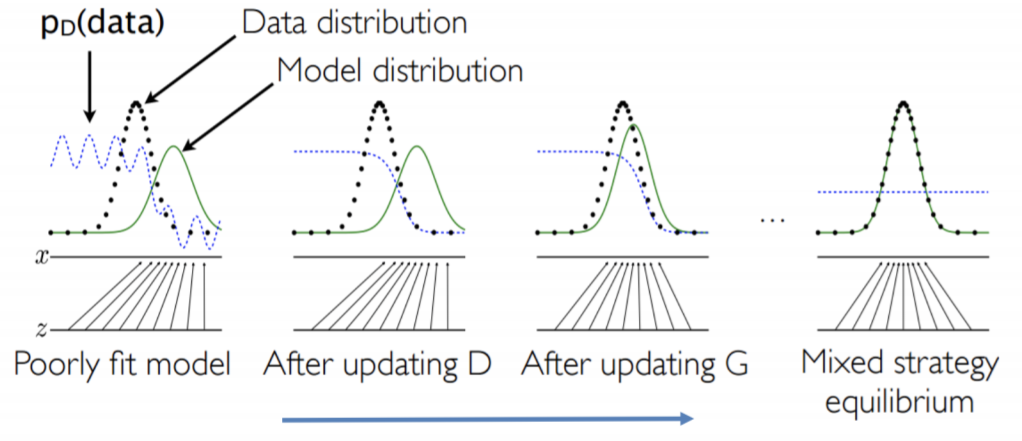
\includegraphics[width=5in,scale=1]{images/GANdist.png}
\caption[Illustration of GAN learning to map uniform noise to the Gaussian distribution]{Illustration of GAN learning to map uniform noise to the Gaussian distribution. source: \citep{gandist}}
\label{fig:gandist}
\end{figure}

The training process involves two objectives
\begin{itemize}
\item The discriminator tries to maximize the probability of identifying real data from the fake data generated by the generator.
\item The generator generates realistic samples to fool the discriminator i.e. the generator tries to minimize the discriminator's probability of classifying real data from the fake data.
Thus the generator and discriminator play a minimax game.
\end{itemize}
 Both networks compete to get better against each other. The objective function V(G,D) of minimax game \citep{goodfellow2014generative} between Discriminator D and Generator G is given by
\begin{equation*}
\underset{G}{min}\underset{D}{max}V(D,G)=\mathbb{E}_{x\sim P_{data}(x)}[log D(x)] + \mathbb{E}_{z\sim P_{z}}(z)[log(1-D(G(z))]
\end{equation*}
where, D(x) is the discriminator's probability estimate that the real instance of the image is real, $\mathbb{E}_x$ is the expected value over instances of real data x, G(z) is the generator's output for the noise z, D(G(z)) is the discriminator's probability estimate that a fake instance of the image is real and $\mathbb{E}_z$ is the expected value over all random noise inputs to the generator.

\section{Conditional GANs}
	Conditional GAN is an extension of the original GAN. Both the generator and the discriminator add additional information y as a condition, y can be any information, such as class labels, image, or music data. The conditional GANs are used in various applications such as image-to-image translation, style transfer, text to image synthesis, etc.
\newline
\begin{figure}[H]
\centering
\includegraphics[width=5in]{images/cgan.jpg}
\caption[Conditional GAN]{Conditional GAN. Source: \citep{gans}}
\label{fig:cgan}
\end{figure}	
	
	 Figures \ref{fig:gan} and \ref{fig:cgan} show the difference between the standard GAN and conditional GAN ie. conditional GAN is realized by sending additional information y to the discriminator and the generator as part of the input layer. Similarly, the objective function of conditional GAN is a two-player minimax game with conditional probability \citep{isola2017image} which is given by
\begin{equation*}
\underset{G}{min} \underset{D}{max} V(D,G)=\mathbb{E}_{x\sim P_{data}(x)} [log D(x|y)] + \mathbb{E}_{z\sim P_{z}}(z) [log(1-D(G(z|y))]
\end{equation*}
where,
$D(x|y)$ is the discriminator's probability estimate that real data instance x is real given the target label y and $G(z|y)$ is the generator's output when given noise z and the target label y.
\section{OCR}
OCR is the computer vision task of localizing and detecting the text in an image. The recent developments in the deep learning approaches revived interests in the OCR problem. Different neural network architectures have been investigated to address the OCR challenge. Before the deep learning era, traditional approaches adopted connected component analysis or sliding window approaches as a solution for OCR. 
\begin{figure}[H]
\centering
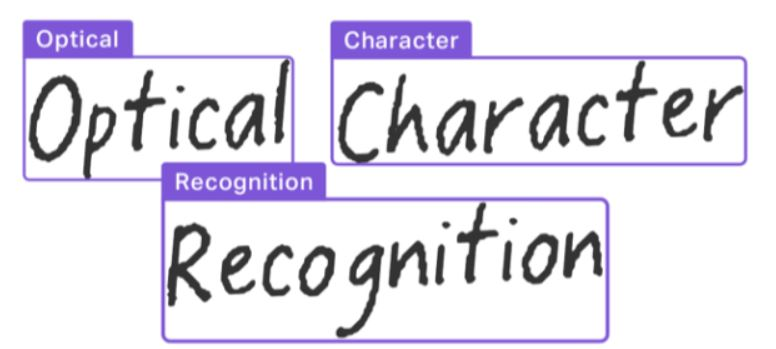
\includegraphics[width=3in,scale=1]{images/ocr.png}
\caption[Optical Character Recognition]{Optical Character Recognition. Source: \citep{ocr}}
\label{fig:neuron}
\end{figure}

The existing methods can be classified into three types:
\begin{enumerate}
\item \textbf{Text detection:} It detects \& localize all the texts in the image. Bounding box coordinates is the output of the text detection.
\item \textbf{Text recognition:} It uses the output of text detection and converts the text into a digital format.
\item \textbf{End to End approach:} They perform both detection and recognition as a single approach.
\end{enumerate} 
\section{Related works}
This section provides an overview of the literature review in several related areas of research. Some of the existing methods for OCR are reviewed under different perspectives which are as follows:
\subsection{General OCR}
	Initially, researchers tried object detection models like faster R-CNN for text detection \citep{nagaoka2017text,zhong2019anchor}. But these algorithms are not very accurate and does not perform well for scene text detection.
\newline	
	
	\cite{tian2016detecting} proposed \gls{ctpn} models utilize the idea of anchoring and \gls{rnn} for sequence labelling. The input is usually passed into the pre-trained models like VGG trained with the ImageNet dataset. The output is then passed to the Bidirectional LSTM. A fully connected layer is used as an output layer which gives the bounding box coordinates for the anchor box, text probability scores and side refinements. The detection is not good for natural scene images, such as curved text and multi-directional text (vertical text).
\newline	
	
	SegLink is proposed especially for long and multi-oriented text. It is similar to the CTPN idea, at first, all parts of the text are found, and then they are connected to form a complete text line \citep{shi2017detecting}. An improved version of the SSD-based network structure is proposed to simultaneously predict two basic elements of text line detection are: segments and links. The segment is actually a bounding box output similar to the \gls{ssd} but added with a direction which is expressed as ($x_b,y_b,w_b,h_b,\theta$) where $x_b, y_b$ represents the center of the segment, $w_b, h_b$ indicates the width and height of the segment and $\theta$ represents the rotation angle of the segment. Links are the connection of segments, i.e, the probability value of whether two boxes are of the same text. One drawback of SegLink is that it cannot detect text lines with large intervals, cannot detect curved text.
\newline
	
	\cite{zhou2017east} proposed \gls{east} uses VGG16/PVANet trained on ImageNet dataset as a feature extractor. The input is passed into the feature extractor and a U-Net architecture is used to merge the feature maps. The output layer consists of probabilities of text in a region and all the bounding box coordinates. The limitation is that the receptive field of EAST is not very large and hence it is not good for detecting lengthy texts.
\newline
	
	The existing text detection methods such as bounding box regression is not accurate for the texts in arbitrary shapes such as curved text, and the segmentation method does not work well when the text is close to each other. In order to solve these two problems, \cite{wang2019shape} proposed a new method called a new \gls{pse}. It works as a segmentation based detector with numerous predictions with for every individual text instance. Thus, the proposed pixel-based segmentation method can accurately locate texts of any shape and detect two text instances even when they are very close. 
\newline
	
	Similar to the above approach, \cite{tian2019learning} proposed a method called Learning Shape-Aware Embedding for Scene Text Detection. The idea is to map image pixels to embedding in the feature space, pixels belonging to the same text instance will be closer to each other in the space, whereas pixels of different text instances will be further away from each other. ResNet-50 is used as a feature extractor. The network output includes the embedded feature map and the mask map of texts. It performs well on three benchmark scene text detection datasets ICDAR15 \citep{icdar}, MSRA-TD500 \citep{msra}, and CTW1500 \citep{yuan2019ctw}.
\newline
	
	\cite{wang2019arbitrary} introduced a method called Arbitrary Shape Scene Text Detection with Adaptive Text Region Representation. It involves two-stage text detection. The first stage is similar to Faster R-CNN. Text proposals are obtained through \gls{cnn} + \gls{rnn} + \gls{roi}. The second stage is to refine the text proposals to make the prediction frame more accurate. The network uses SE-VGG16 as a feature extractor. Experiments show that \gls{se} Block can improve performance. The main advantage of the proposed method is that it uses adaptive points instead of fixed points to represent a text box. The previous methods used fixed points to represent the text box, but the number of points for horizontal text, multidirectional text, and curved text is not the same. So, the points to represent the text box are adapted to detect text of various shapes. It uses the \gls{lstm} network to learn how many points should be used to represent the text box.
\newline
	
	Similar to SegLink, \cite{baek2019character} proposed \gls{craft} that detects text area by identifying single character (character region score) and connection between each characters (affinity score). The network structure is similar to the EAST network structure: the feature extraction backbone network part uses VGG-16 with batch normalization; the feature decode module is similar to U-Net, and it also uses a top-down feature aggregation method; the network finally outputs two channel feature map, that is, region score map and affinity score map in the form of the heat map. This thesis uses the CRAFT pre-trained model for text detection and \cite{baek2019wrong} proposed model for text recognition.

\subsection{OCR for steel type plates}

	Similar to steel type plate recognition, many research works have been published to extract text from the vehicle license plate, forms, and documents \citep{duan2005building,zang2015vehicle,impedovo2012fundamentals,
milewski2006extraction,laroca2018robust}. Several deep learning and computer vision algorithms exist to solve these problems. But the existing approach would fail for our steel type plate images since the complexity of our problem is relatively higher. 
Before the deep learning era, there have been several classical research works done to improve the accuracy of OCR for steel type plates. Some of the approaches similar to our problem are discussed below: 
\newline
	
	\cite{novak2013recognition} used fuzzy logic methods for the recognition of distorted characters printed on metal. \cite{yu2017engraving} proposed a technique that involved image processing with a series of mathematical and morphological treatments for metal surface engraving character detection.  \cite{xiang2018metal} proposed a technique called \gls{msc}. They combined and fused the images of the steel plates of the same scene from multi-direction and different illuminations to improve the character recognition of metal stamped characters. \cite{raka2019ocr} proposed an algorithm based on \gls{knn} for reading embossed text from credit/debit cards. After preprocessing steps, they locate the credit/debit card number and split it into individual characters. They created a dataset by manually sorting characters from 0 - 9 and then trained the OCR model with its corresponding label using KNN. These classic approaches are performing basic image manipulation operations like image binarization, thresholding, segmentation and other morphological processes to increase the quality of the original image. 
\newline

	Recent advancements in computer vision have given a set of new possibilities to tackle advanced recognition problems. \cite{patil2015engraved} proposed a computer vision technique to identify texts from the engine and chassis parts.  With the success of CNNs in the image classification \citep{hinton2012improving,simonyan2014very}, Segmentation \citep{girshick2014rich}, Object Detection \citep{russakovsky2015imagenet}, it is combined with recurrent networks along with attention mechanism for solving OCR problem. 
\newline

	\cite{bui2017selecting} proposed an algorithm that automatically selects the preferred pre-processing methods to be applied to a document image to maximize OCR performance for the processed image. They used 21 different such possible combinations to pre-process the image. Their approach achieved a good improvement in the performance of OCR. But the main drawback is that the possible pre-processing options were limited. Also, it does not suit our requirements.  
\newline

	Similar to our approach, \cite{hu2019embossed} used CNN for enhancing the character recognition of embossed characters of the shoe soles. Their research focussed only on image enhancement and did not care about the character recognition part.
	
\subsection{GANs in OCR}
	 Using standard GANs, \cite{karras2017progressive} generated highly realistic human faces trained with the celebrity dataset while \cite{jin2017towards} generated faces of anime characters. Likewise, \cite{brock2018large} demonstrated the ability of GANs to generate synthetic images of objects that are not differentiable from the real images using the BigGAN technique. Works such as \citep{zhang2017stackgan,reed2016learning,reed2016generative,dash2017tac} used conditional GANs to generate images given its description as text which is popularly known as text-to-image translation.
\newline

	Large scale annotated datasets are required for the development of robust deep learning models, especially for CNN. Acquiring such datasets is always challenging in cases like medical images. Hence, \cite{frid2018gan} used GANs to generate synthetic medical images as a data augmentation technique to increase the performance of CNN in classifying images of liver lesions. Similarly, \cite{fiore2019using} used GAN for improving the effectiveness of classifying credit card fraud detection. Even though it was a binary classification problem, the dataset was heavily imbalanced i.e. the interested class was represented significantly lesser than the other. Synthetic images were generated for the imbalanced class as an alternative to oversampling techniques.
\newline
	
	For our case, since the goal was to generate a clear image from noisy steel type plate images in order to maximize the OCR performance, it was realized that one way to go about solving this problem is by using a generative adversarial image. 
Some of the research works using GANs for improving character recognition are presented below:
\newline

	\cite{hosangadi2019ocr} proposed a method that uses DCGAN for enhancing the image quality of documents to improve the OCR performance. Their model uses an encoder trained to learn the latent representation of a low-quality image. The latent representation is then passed as an input to the conditional GAN generator which is trained to produce a high-quality image.
\newline
	
	 \cite{lat2018enhancing} proposed a super-resolution based solution for improving the OCR accuracy using GAN. They used SRGAN to convert the low resolution (scanned at as low as 75dpi) document images into super-resolved texts and then passed it into the OCR engine. 
\newline
	 
	 Similarly, \cite{karimi2020illegible} developed a model called Handwritten-to-Machine-Print Generative Adversarial Network (HW2MP-GAN) to transform the handwritten text to machine-printed text. Their model utilizes sliced Wasserstein distance and U-Net architecture for better quality image-to-image translation. These approaches work well for printed documents and have shown to improve the accuracy of OCR.
\newline

	In summary, we list out the papers that especially influenced this work. The proposed overall framework uses a GAN generator model and an OCR engine. For GAN, the best generator model is selected among the three image-to-image translation GANs: i) \cite{isola2017image} proposed a pix2pix GAN , ii) \cite{CycleGAN2017} proposed CycleGAN  and iii) \cite{stoller2019training} proposed FactorGAN. For OCR engine, the text detection uses CRAFT approach \citep{baek2019character} and the text recognition uses \cite{baek2019wrong} proposed text recognition model.